\chapter{Grafen}
	Zgodnie z najnowszą definicją grafen to: ,,Cienka monowarstwa zbudowana z atomów węgla,
ułożonych w dwywymiarowej sieci o stukturze plastra miodu. Grafen jest podstawowym budulcem
dla materiałów grafitowych o innych wymiarach. Może być zwinięty tworząc zerowymiarowe fullereny,
zrolowany w jednowymiarowe nanorurki lub spiętrzony w stos tworząc trójwymiarowy grafit''	
\footnote[1]{(odnośnik do Geim, A. K. and Novoselov, K. S. (2007). "The rise of graphene". Nature Materials 6 (3): 183–191. 					Bibcode:2007NatMa...6..183G. doi:10.1038/nmat1849. PMID 17330084.)}

	Ta definicja pokazuje, że grafen stanowił ważny materiał, jeszcze zanim udało się znaleźć metodę jego otrzymywania, \footnote[2]{tutaj o początkach grafenu} ponieważ odgrywał ważną rolę w modelowaniu właściwości innych materiałów zbudowanych z węgla (fullereny, nanorurki).
	
Poniższy rozdział ma na celu przybliżenie własności grafenu, dzięki którym możliwe
zastosowania stanowią o dzisiejszym, niesamowitym zainteresowaniu ze strony naukowców z całego świata. Dodatkowo
zostanie zaprezentowana i omówiona metoda jego otrzymywania, w której upatruje się 
największe nadzieje na otrzymywanie przemysłowych ilości tego niezwykłego materiału.
Na sam koniec przedstawione zostaną niektóre z wielu zastosowań grafenu z naciskiem na
tranzystory polowe z kanałem grafenowym, które stanowią główną oś niniejszej pracy.

\newpage

	\section{Struktura atomowa i własności mechaniczne}
	Jeżeli skupimy się na pojedynczym atomie węgla tworzącym grafen, wtedy okaże się, że 
	mamy do czynienia z hybrydyzacją typu $\mathrm{sp^2}$. Takie oddziaływanie między
	orbitalami s i p prowadzi do powstania bardzo silnych wiązań typu $\sigma$ pomiędzy
	sąsiednimi atomami węgla. Te wiązania mają, zgodnie z zasadą Puliego, zapełnione 
	powłoki elektronowe i tworzą głębokie pasmo walencyjne. Długość tego wiązania wynosi
	1,42 Å i leżą one w jednej płaszczyźnie. To te wiązania decydują o tak dużej stabilności tego
	układu i o jego niezwykłych właściwościach mechanicznych. Wygląd tak powstałej sieci widoczny jest na 
	rysunku \ref{fig:siec_grafenu}. 
	
	\vspace{-10pt}
	\begin{figure}[ht]
	\centering
	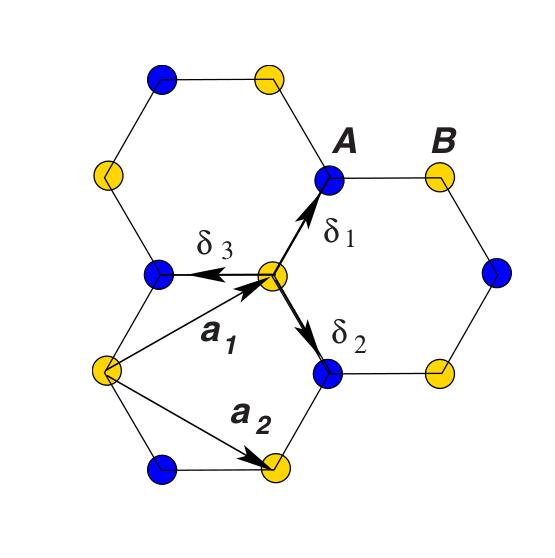
\includegraphics[width=0.50\textwidth]{./Rozdzial_2/obrazki/Siec_grafen.jpg}
	\caption{Sieć atomowa grafenu}
	\label{fig:siec_grafenu}
	\end{figure}
	\vspace{-10pt}

	Na rysunku możemy zobaczyć, że sieć grafenu zbudowana jest z dwóch dwuwymiarowych sieci Bravais'ego (kolory 
	niebieski i żółty), oznaczone literami A i B. Dodatkowo widoczne są wspomniane wcześniej trzy wiązania $\sigma$.
	Warto też wspomnieć o dwóch wektorach a$_1$ i a$_2$, tworzących pojedynczą sieć Bravais'ego. O ile nie mają one,
	większego znaczenia dla samego opisu grafenu, o tyle warto o nich wspomnieć w kontekście nanorurek węglowych. Dzięki
	wielokrotnościom tych wektorów określa się tak zwany wektor chiralności nanorurki. Dzięki temu można poznać charakter
	nanorurki (metaliczny czy półprzewodnikowy).
	
	Jako wynik takiej budowy sieci grafenu, jest on bardzo wytrzymały. Teoretycznie 100 razy bardziej wytrzymały niż
	stal o takiej samej grubości. Mimo wszystko jest on też bardzo lekki. Istnieje bardzo obrazowe
	porównanie obu tych właściwości. Gdyby wytworzyć grafenowy hamak o powierzchnii 1 m$^2$, to taki hamak byłby
	w stanie wytrzymać 4-kilogramowego kota. Jednocześnie sam hamak  ważyłby mniej niż jego pojedynczy wąs. 
	Dokładniej ważyłby 0.77 mg, jest to $10^{5}$ razy mniej niż waga arkusza papieru o tej samej powierzchni.

\section{Własności elektronowe}
	Po utworzeniu 3 par typu $\mathrm{sp^2}$ pozostaje jeden orbital typu p, będący prostopadły do
	powierzchni tworzonej przez wiązania typu $\sigma$. Wraz z niesparowanymi orbitalami typu p pochodzącymi od
	 sąsiednich atomów,  tworzy on zdelokalizowane wiązanie typu $\pi$
	Wiązania typu $\pi$ są znacznie słabsze niż wiązania typu $\sigma$. Dodatkowo są one 
	wypełnione tylko w połowie elektronami. Dlatego właśnie to wiązanie decyduje o niezwykłych właściwościach 
	elektronicznych grafenu.

	\subsection{Struktura pasmowa}
	Na początku omówienia właściwości elektronicznych grafenu warto przedstawić sieć odwrotną dla tego materiału.
	Schemat pierwszej strefy Brillouina znajduje się na rysunku \ref{fig:siec_odwrotna}.
	
	\vspace{-10pt}
	\begin{figure}[ht]
	\centering
	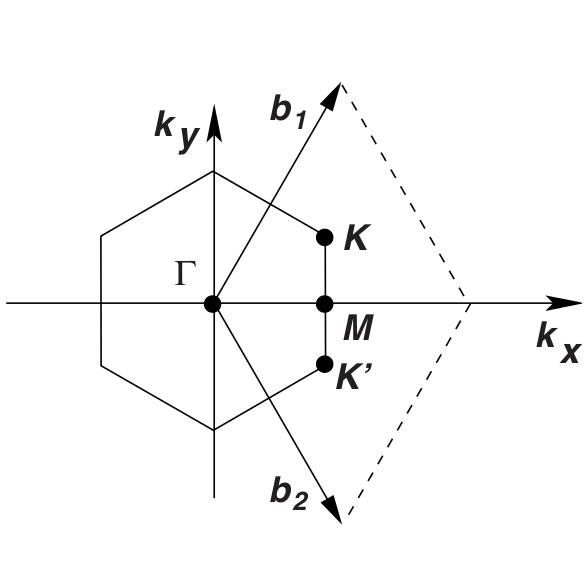
\includegraphics[width=0.50\textwidth]{./Rozdzial_2/obrazki/Siec_odwrotna.jpg}
	\caption{Sieć odwrotna grafenu}
	\label{fig:siec_odwrotna}
	\end{figure}
	\vspace{-10pt}
	Zaznaczone są na nim punkty wysokiej symetrii ($\Gamma$, K i M). Dodatkowo pokazane zostały wektory b$_1$ i b$_2$, 
	opisujące sieć odwrotną. Warto zauważyć, że sieć odwrotna bardzo przypomina sieć atomową. Z geometrycznego punktu
	widzenia sieć odwrotna jest to obraz sieci atomowej obrócony o 30$^o$. 
	Operując w sieci odwrotnej można wyprowadzić zależność energii od położenia na płaszczyźnie wektora k. Najprostszą
	metodą otrzymania takiej zależności jest metoda ciasnego wiązania (\textit{ang. Tight-binding method}). Prowadzi ona
	do następującej zależności energii:
	\begin{equation}
    		E(\vec k)_{\pm}=\pm t \sqrt{3+f(\vec k)} - t'f(\vec k)
		\label{equ:energia}
	\end{equation}
	\begin{equation}
    		f(\vec k)= 2\cos({\sqrt{3}k_y a}) + 4\cos \left (\frac{\sqrt{3}}{2} k_y a \right )\cos \left (\frac{3}{2}k_xa \right )
	\end{equation}

	Oznaczenie t występujące w zależności \ref{equ:energia} jest to energia przeskoku pomiędzy danym atomem a 
	jego najbliższym sąsiadem (zmiana podsieci). Natomiast t' jest to energia przeskoku pomiędzy następnym najbliższym
	sąsiadem. Wartość t$\approx$2,8 eV, natomiast t'$\approx$0,2 eV. Na podstawie oby tych zależności 
	\ref	{equ:energia}, został narysowany wykres zależności energii w pierwszej strefie Brillouina, który zostął 
	przedstawiony na rysunku \ref{fig:Struktura_pasmowa}.
	Ze wzoru \ref{equ:energia} wynika też, że jeżeli energia t' jest różna od zera, wtedy pasmo przewodnictwa i 
	walencyjne są asymetryczne.
	Dodatkowo zaznaczony został obszar w pobliżu punktu K.
	
	%\vspace{-10pt}
	\begin{figure}[t]
	\centering
	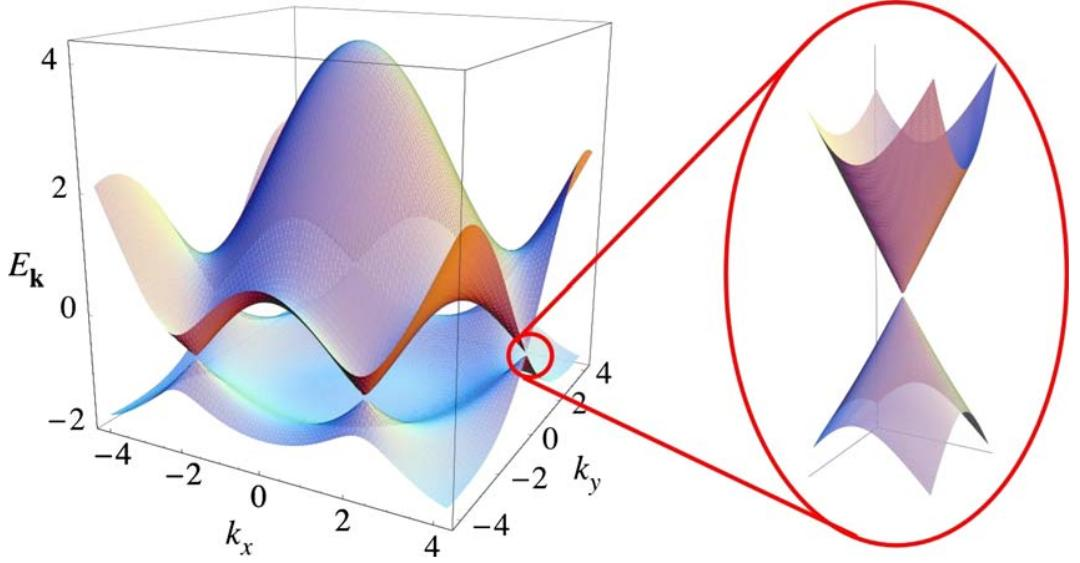
\includegraphics[width=0.80\textwidth]{./Rozdzial_2/obrazki/Struktura_pasmowa.jpg}
	\caption{Struktura pasmowa grafenu}
	\label{fig:Struktura_pasmowa}
	\end{figure}
	%\vspace{-10pt}

	Wyróżniony obszar to tak zwany stożek Diraca. Jest to w zasadzie najciekawsze miejsce na krajobrazie pasmowym z 
	co najmniej dwóch powodów. Po pierwsze jest to miejsce, gdzie stykają się pasma przewodnictwa i walencyjne. 
	Po drugie w pobliżu punktu K mamy do czynienia z liniową zależnością energii od wektora falowego. 
	Najczęściej tą relację w przybliża się w poprzez rozwinięcie w szereg i ograniczenie 
	się do pierwszego wyrazu liniowego:
	\begin{equation}
    		E(\vec k) = \pm v_F|\vec k|
		\label{equ:liniowa_dyspersja}
	\end{equation}
	Gdzie $\vec k = \vec K + \vec q$ i jednocześnie $|\vec q| << |\vec K|$. $v_F$ Jest to tak zwana prędkość Fermiego
	i wynosi $v_F = \frac{3ta}{2}$, a co do wartości $v_F \approx 10^6 \frac{m}{s}$. Taki wynik jest bardzo różny 
	od typowej zależności dla materiałów stosowanych w elektronice, ponieważ zazwyczaj zależność energii jest 
	funkcją kwadratową wektora falowego. 
	Liniowa zależność świadczy o występowaniu cząstek bez masowych, zwanych bez masowymi 
	fermionami Diraca. Taka zależność
	została potwierdzona eksperymentalnie. Takie kwazicząstki są bardziej podobne do fotonów niż do elektronów. 
	To właśnie ta właściwość nośników występujących w grafenie stanowi o jego niespotykanych pośród innych materiałów
	właściwościach.
	
	\subsection{Ruchliwość}
	Dodatkowo bezmasowość nośników stanowi o bardzo wysokich ruchliwościach zarówno dla przewodnictwa dziurowego 
	jak i elektronowego, co ważne nawet w temperaturach pokojowych. Jest to powszechnie uważane za największą
	zaletę tego materiału.

	Ruchliwości z zakresu 10 000 - 15 000  $\mathrm{\frac{cm^2}{V\cdot s}}$ są typowe dla grafenu eksfoliowanego
	na podłożu z SiO$_2$.\footnote{Chen, J-H., Jang, C., Xiao, S., Ishigami, M. \& Fuhrer, M. S. Intrinsic and
extrinsic performance limits of graphene devices on SiO2. Nature Nanotech.3, 206–209 (2008).}
Jednak teoretyczne ograniczenia dla tego typu układów zostały przewidziane na 40 000 - 70 000  
	 $\mathrm{\frac{cm^2}{V\cdot s}}$ \footnote{to co wyżej i Chen, F., Xia, J., Ferry, D. K. \& Tao, N. Dielectric screening enhanced
performance in graphene FET. Nano Lett. 9, 2571–2574 (2009).}

	Co więcej przy założeniu braku defektów struktury i rozpraszaniu tylko na fononach akustycznych, przewidywana
	ruchliwość wynosi 200 000 $\mathrm{\frac{cm^2}{V\cdot s}}$ \footnote{Morozov, V. S. et al. Giant intrinsic carrier mobilities in graphene and its bilayer.
Phys. Rev. Lett. 100, 016602 (2008).}. Co ciekawe donosi się o zmierzonej ruchliwości dla grafenu zawieszonego swobodnie
	wynoszącej 10$^6$ $\mathrm{\frac{cm^2}{V\cdot s}}$ \footnote{Geim, A. Graphene update. Bull. Am. Phys. Soc. 55, abstr. J21.0004,
http://meetings.aps.org/link/BAPS.2010.MAR.J21.4 (2010).}. 
	Dla grafenu otrzymanego metodą CVD na folii niklowej i przetransferowanego na podłoże, zmierzona ruchliwość 
	przekraczała 3 700 $\mathrm{\frac{cm^2}{V\cdot s}}$. \footnote{Kim, K-S. et al. Large-scale pattern growth of graphene films for stretchable
transparent electrodes. Nature 457, 706–710 (2009).} Donosi się też o uzyskaniu grafenu wytwarzanego metodą CVD
	dającego średnią ruchliwość wynoszącą 7 000 $\mathrm{\frac{cm^2}{V\cdot s}}$.\footnote{http://meetings.aps.org/Meeting/MAR13/Session/B6.6}
	Z punktu widzenia niniejszej pracy największe znaczenia mają wyniki otrzymywane dla grafenu CVD, ponieważ próbki
	tego typu były mierzone podczas pomiarów.
	
	Te liczby robią wrażenie. Jednak należy na nie patrzeć trochę z dystansem porównując je z typowymi materiałami
	półprzewodnikowymi. Głównym powodem tego jest brak przerwy energetycznej. Ten problem zostanie omówiony szerzej
	w późniejszym podrozdziale, jednak problem został zaznaczony już tutaj.


	\subsection{Minimalna przewodność i gęstość stanów}
	Inną ważną właściwością jest minimalna przewodność grafenu występująca również blisko punktów Diraca. Według 
	rozważań teoretycznych przewodność ta powinna wynosić $\mathrm{4\frac{e^2}{h}}$ (4 wynika z czterokrotnego 
	zdegenerowania). Ta wartość jest poparta wynikami teoretycznymi \footnote[9]{Geim, A. K. and Novoselov, K. S. (2007). "The rise of graphene". Nature Materials 6 (3): 183–191. Bibcode:2007NatMa...6..183G. doi:10.1038/nmat1849. PMID 17330084.}. Należy jednak pamiętać, że grafen na podłożu SiO$_2$, wykazuje pewne pofalowanie co znajduje swoje 
	odzwierciedlenie jako pojawienie się lokalnych nośników i co z tym związane: zwiększenie tej wartości. 
	Istnienie takiej minimalnej przewodności związane jest z funkcją gęstości stanów w grafenie. Dla uproszczenia 
	załóżmy, że pasma przewodnictwa i walencyjne są symetryczne. Wykres dla takiego założenia przedstawia obrazek
	\ref{fig:gestosc_stanow}.

	\vspace{-10pt}
	\begin{figure}[ht]
	\centering
	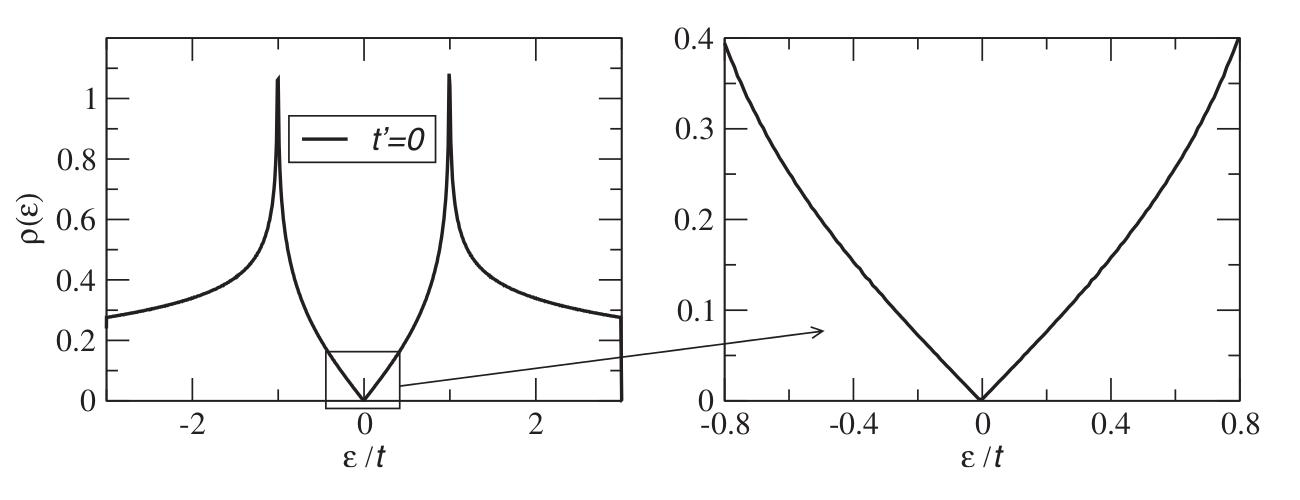
\includegraphics[width=0.90\textwidth]{./Rozdzial_2/obrazki/gestosc_stanow.jpg}
	\caption{Gęstość stanów}
	\label{fig:gestosc_stanow}
	\end{figure}
	\vspace{-10pt}

	Założenie o symetrii pasm jest w pełni akceptowalne pod warunkiem ograniczenia się
	 do punktów z bliskiego sąsiedztwa punktów Diraca w przestrzeni wektora falowego. W takim reżimie zależność
	energii od wektora falowego jest liniowa, zgodnie ze wzorem \ref{equ:liniowa_dyspersja}. 
	Dodatkowo funkcję gęstości stanów można przedstawić przy pomocy następującego wzoru:
	\begin{equation}
  	  \rho(E)=\mathrm{\frac{2A_c}{\pi}}\frac{|E|}{{ v_F^2}}
	\label{equ:gestosc_stanow}
	\end{equation}
	Co zostało przedstawione w prawej części wykresu \ref{fig:gestosc_stanow}. Co świadczy o dobrym przybliżeniu 
	gęstości stanów równaniem \ref{equ:gestosc_stanow} dla dostatecznie małych energii. Wzór ten odpowiada gęstości
	stanów w komórce elementarnej. Uwzględniono w nim już poczwórną degenerację.

	\subsection{Przerwa energetyczna}
	Ze struktury pasmowej i funkcji gęstości stanów wynika, że grafen jest materiałem mającym charakter półmetalu.
	Jest to o tyle ważne, że nie posiada on przerwy energetycznej. Przez wielu jest to uważane za główną wadę
	grafenu, co dyskwalifikuje go w ewentualnym zastąpieniu krzemu w dzisiejszej masowej produkcji elektroniki, która
	 oparta
	jest na technologii CMOS (\textit{ang. Complementary Metal-Oxide-Semiconductor}). Taki brak przerwy powoduje, 
	że urządzenia zbudowanego z użyciem grafenu jako głównego komponentu, nie dało by się po prostu wyłączyć, a jedynie
	sprowadzić do stanu minimalnego przewodnictwa. Wiąże się to z dużymi stratami mocy co oczywiście z punku widzenia
	ewentualnych urządzeń elektronicznych jest niedopuszczalne. 
	Jednak trwają usilne próby mające na celu otwarcie przerwy energetycznej grafenu. Jak na razie przedstawione zostały
	trzy główne metody. Są nimi: wytworzenie nanowstążki\footnote{\textit{nanoribbon}}, zastosowanie dwuwarstw, 
	wytworzenie silnego odkształcenia jednoosiowego.\footnote{Tutaj nawstawiać odnośników z grafenowego tranzystora}
	
	Oczywiście każda z tych metod ma swoje wady. Nanowstążki muszą być bardzo wąski (rzędu kilkudziesięciu nanometrów),
	dodatkowo, co bardzo ważne, muszę mieć bardzo dobrze zdefiniowane brzegi (nie ma znaczyenia czy zig-zag, czy 
	armchair). Jest to niezwykle trudne zadanie, co ogranicza je w przemysłowym zastosowaniu. Dodatkowym minusem jest
	znaczne zmniejszenie ruchliwości (głównej zalety grafenu) do poziomu poniżej 200 $\mathrm{\frac{cm^2}{V\cdot s}}$
	dla nanowstążek o szerokości 1-10 nm, \footnote{26,62 grefenowy tranzystor} oraz 1 500 
	$\mathrm{\frac{cm^2}{V\cdot s}}$ dla nanowstążki o szerokości 14 nm\footnote{45, grafenowy tranzystor}. 
	Dlatego pozwalając na upodobnienie grafenu do typowych materiałów półprzewodnikowych skutkuje zniszczeniem
	jego największej zalety, ogromnej ruchliwości.
	
	Jeżeli chodzi o dwuwarstwę to dużym problemem staje się to, że pasma zaczynają stawać się paraboliczne. Przypominają
	te z typowych półprzewodników. Dodatkowo przerwa otwarta w ten sposób jest dość wąska i wynosi ok 200-250 meV.
	Znowu widoczne jest pogorszenie się ruchliwości.

	Ostania metoda jest chyba najciekawsza. Zakłada ona silne, globalne odkształcenie jednoosiowe materiału. 
	Przewiduje się, że odkształcenie powinno wynosić powyżej 20\%. Na pierwszy rzut oka takie rozwiązanie wydaje
	się być najprostsze ze wszystkich. Jednak trudno jest je wykonać w praktyce. Dodatkowo nie wiadomo jaki wpływ
	mają odkształcenia nieosiowe lub lokalne na przerwę w grafenie. Na razie są to rozważania teoretyczne.

	Podsumowując choć jest znanych co najmniej trzy metody otwarcia przerwy energetycznej w grafenie to jednak
	należy założyć, że póki co nie mają one znaczenia z punktu widzenia zastosowania ich do ewentualnej 
	technologii produkcji przyrządów elektronicznych.
	


	\subsection{Efekty środowiskowe}
	Innym problemem jest oddziaływanie grafenu z otoczeniem. Ze względu na swoje rozmiary, grafen jest podatny
	na wszelkiego rodzaju zanieczyszczenia osiadające na jego powierzchni. Oczywiście tę wadę można przekuć w 
	zaletę, np. wykorzystując ją do produkcji różnego rodzaju detektorów, nawet pojedynczych cząsteczek
	\footnote{odniesienie}. Niemniej jednak w zastosowaniach w charakterze tranzystorów jest to dość poważna wada. 
	Chociażby z tego względu, że chcielibyśmy, aby nasze urządzenia posiadały tak stabilne parametry jak to tylko
	możliwe.
	Dodatkowo należy pamiętać, że same metody wytwarzania pozostawiają po sobie różnego rodzaju zanieczyszczenia, 
	które w ogólności zachowują się jak domieszki. Dlatego proces produkcji grafenu praktycznie zawsze 
	wymaga jakiegoś dodatkowego
	etapu, mającego zmniejszenie liczby zanieczyszczeń. Metody te nie są też doskonałe i otrzymany nimi grafen często
	posiada wady strukturalne (w zasadzie nie dotyczy to tylko grafenu otrzymywanego metodą eksfoliacji) .
	
	Jedną z metod mających na celu poprawę jakości, jest tak zwane czyszczenie grafenu poprzez
	 wygrzewanie gotowego urządzenia prądem elektrycznym
	o dużej gęstości, najczęściej w próżni. Taki proces zostanie opisany dokładniej w trakcie omawiania zagadnień 
	dotyczących tranzystorów z kanałem grafenowym.
	
	Innym problemem są zaburzenia w wysokości grafenu, spowodowane np. oddziaływaniem z podłożem. Takie fluktuacje 
	wysokości zaburzają delikatną strukturę wiązań typu $\pi$, które jak już zostało wspomniane wcześniej mają 
	najbardziej znaczący 
	wpływ na własności elektronowe grafenu. Niestety nie ma na razie prostego sposobu rozwiązania tego problemu.
	Dodatkowo takie odkształcenia powodują również powstanie lokalnych naprężeń, co jak pokazano wcześniej może
	prowadzić nawet do otwarcia przerwy energetycznej.

	Problematyczne są również wszelkie defekty struktury (pochodzące głównie z niedoskonałości procesu wytwarzania). 
	Ich występowanie ma znaczący wpływ na pogorszenie się
	ruchliwości, poprzez zwiększenie rozpraszania na właśnie tych defektach. Dodatkowo takie defekty mogą powodować
	efekty tożsame z domieszkowaniem grafenu, co jest również niepożądanym efektem. 
	Co ciekawe istnieją metody na poprawę
	jakości strukturalnej grafenu. Jedną z nich jest bombardowanie powierzchni grafenu atomami węgla w odpowiednich
	warunkach. Podczas tego procesu dochodzi do samonaprawy defektów polegających na braku atomu w węźle.
	Co ciekawe taka samonaprawa możliwa jest również w obecności niektórych gazów lub nawet bez żadnej "pomocy z zewnątrz" w postaci ciepła, ciśnienia, bombardowania cząstkami. \footnote{Graphene Reknits Its Holes}
	Jest to naprawdę ciekawa właściwość tego materiału raczej niespotykana nigdzie indziej.

	Podsumowując, wszystkim tym problemom możemy przyporządkować trzy podstawowe wpływy na własności elektronowe
	grafenu. Są nimi: pojawienie się przerwy energetycznej, degradacja ruchliwości i wreszcie efekty, które można 
	utożsamiać z domieszkowaniem.
	Problem przerwy energetycznej był już omawiany oddzielnie dlatego nie będzie omawiany teraz.
	Degradacja ruchliwości jest przede wszystkim następstwem wytworzenia przerwy energetycznej w grafenie, 
	defektami lub domieszkami. Ogólnie mówiąc wszytko co może zwiększyć rozpraszanie elektronów będzie 
	prawdopodobnie degradowało ruchliwość w grafenie.
	Efekty domieszkowania są o tyle uciążliwe, że mają bardzo duży wpływ na własności gotowych urządzeń.
	Jak już wspomniano wcześniej grafen bardzo łatwo ulega domieszkowaniu co powoduje znaczne przesunięcia 
	poziomu Fermiego w strukturze pasmowej. Jest to o tyle istotne, że nawet w obecności normalnej 
	atmosfery widoczny jest ten efekt. Prawdopodobnie głównym winowajcą jest tutaj wszechobecna wilgoć
	i wytwarzanie się cienkiej warstewki wody na powierzchni grafenu, co w połączeniu z ewentualnymi 
	większymi zanieczyszczeniami prowadzi do znacznych przesunięć poziomu Fermiego.
	Dla idealnie czystego i idealnie strukturalnego grafenu, poziom
	Fermiego znajduje się dokładnie na styku pasma przewodnictwa i walencyjnego, w stożku Diraca.
	Zmiana tego poziomu powoduje bardzo duże zmiany w charakterystykach np. tranzystorów typu FET (
	\textit{ang. Field Effect Transistor}), co jest niedopuszczalne dla przemysłu.
	Jest to tematyka dość obszernie porusza w niniejszej pracy, dokładniej w części eksperymentalnej.

	\subsection{Inne właściwości}
		
	Oczywiście grafen posiada wiele różnych innych właściwości czyniących go bardzo pożądanym materiałem. Do nich należą między innymi : wysoka przewodność cieplna \footnote{przewodność cieplna} oraz mała absorbcja \footnote{mała absorbcja} 
	światła z zakresu widzialnego. Ze względu na skończoną objętość niniejszej pracy zdecydowano o nie rozwijaniu 
	tych właściwości jako mało istotnych z punktu widzenia zakresu materiału, o którym traktuje niniejsza praca.
	
\section{Metody otrzymywania grafenu}
	Na dzień dzisiejszy znanych jest już kilka metod otrzymywania grafenu na potrzeby różnych zastosowań. Iskrą 
	zapalną dla poszukiwań takich metod stało się doniesienie przez grupę naukowców z Manchesteru o opracowaniu
	metody otrzymywania tego materiału \footnote{Tutaj odniesienie do pierwszej pracy}. Wcześniej panowało
	powszechne przekonanie, że grafen jako materiał dwuwymiarowy nie może istnieć w takiej postaci, ze względu
	na zbyt duże oscylacje termicznie poszczególnych atomów co w konsekwencji miałoby prowadzić do jego niestabilności.
	Był to przez długie lata główny powód dla, którego sprawa grafenu stanowiła tak zwaną "ziemię niczyją".
	Po 2004 roku kiedy okazało się, że jednak grafen jest stabilny termodynamicznie i istnieje metoda jego otrzymywania,
	działalność twórcza wielu naukowców zwróciła się w jego stronę. Dlatego też w stosunkowo krótkim czasie
	powstało wiele różnych metod otrzymywania. W niniejszym podpunkcie zaprezentowana zostaną metody 
	najbardziej typowe i dające stosunkowo najlepsze rezultaty. Warto jednak podkreślić, że próbki
	otrzymane różnymi metodami różnią się od siebie.

	\subsection{Eksfoliacja}
	
	Jak zostało wspomniane, metoda eksfoliacji jest pierwszą metodą otrzymywania grafenu w sposób powtarzalny.
	Została ona przedstawiona przez grupę naukowców z Manchesteru w 2004 roku. Jako ciekawostkę można powiedzieć,
	że przynajmniej w początkowej fazie, prace nad nią należały do tak zwanych "piątkowych projektów". Dopiero, 
	gdy okazało się, że faktycznie możliwe jest wytworzenie grafenu tą metodą rozpoczęto poważne prace nad nią.
	
	Ogólnie metoda opiera się na fakcie, że grafit jest materiałem zbudowanym z gotowych, niezliczonych warstw 
	grafenowych. Wystarczy je tylko od siebie rozseparować. Dodatkowo wiadomo, że atomy w warstwach grafenu 
	są ze sobą silnie związane wiązaniami typu $\sigma$. Natomiast poszczególne warstwy są ze sobą związane 
	przy pomocy dużo słabszych wiązań Van der Waalsa. 
	Do separacji warstw wykorzystano taśmę klejącą. Po nałożeniu na taśmę fragmentu grafitu, dokonywano wielokrotnych
	złożeń, przy każdym złożeniu rozdzielając warstwy. Po bardzo dużej liczbie takich złożeń taśmę z warstwami 
	umieszczano w acetonie gdzie następował rozkład taśmy i kleju. Otrzymano warstwy grafenowe zawieszone w acetonie.
	Kolejnym krokiem było umieszczenie ich na podłożu krzemowym, pokrytym SiO$_2$ o odpowiedniej grubości.
	Grubość tlenku ma tutaj zasadnicze znaczenie ze względu na absorbcję światła przez grafen. Dla tlenków
	o grubościach 10 nm i 300 nm obserwuje się maksymalny kontrast pomiędzy obszarem pokrytym grafenem i obszarem 	
	podłoża.Ten rodzaj eksfoliacji nazywany jest mokrym, ze względu na użycie rozpuszczalnika pomiędzy procesem 
	separacji a transferu.

	Po około roku metoda została ulepszona przez usunięcie etapu rozpuszczania taśmy w acetonie, a transferu 
	dokonuje się bezpośrednio z taśmy klejącej. W tym przypadku mówi się o suchej eksfoliacji.
	Po procesie transferu, następuje czasochłonny etap poszukiwań pojedynczych warstw. Do tego celu używany jest
	mikroskop optyczny dysponujący odpowiednim powiększeniem. Powiększenie jest niezbędne ze względu na małe 
	rozmiary otrzymywanych warstw. W tym momencie ujawnia się największa wada tej metody. Nie może być mowy
	o jakiejkolwiek powtarzalności. Próbki zazwyczaj są małe, rzędu pojedynczych mikrometrów, choć donosi się
	o warstwach grafenu otrzymanych tą metodą rzędu milimetrów i widocznych gołym okiem na powierzchni podłoża.
	Drugą wadą tej metody jest cena tak pozyskiwanego materiału, z uwzględnieniem znikomej wydajności i 
	ogromu czasu potrzebnego na zlokalizowanie odpowiedniej warstwy.

	Jednak ta metoda ma niezaprzeczalną zaletę. Grafen otrzymany dzięki niej jest bardzo wysokiej jakości 
	strukturalnej, w zasadzie najlepszej. Dzięki czemu jest bardzo pożądanym do celów naukowych. 
	Dodatkowo do jego wytworzenie nie są potrzebne ani wyspecjalizowany sprzęt. Ze względu na prostotę
	metodę można stosować nawet w warunkach domowych.
	Niestety wady tej metody całkowicie eliminują ją w zastosowaniach przemysłowych.

	Warto wspomnieć, że sukces tej metody otworzył przed naukowcami możliwości badania również innych 
	materiałów warstwowych np. siarczku molibdenu, lub siarczku wolframu. Oba te materiały są bardzo
	obiecującymi, wschodzącymi materiałami dla nanoelektroniki.


	\subsection{Epitaksja na węgliku krzemu}

	\subsection{Metoda CVD}
	
		\paragraph{Opis metody}
		\paragraph{Badania strukturalne grafenu}
	\section{Zastosowania}
